%versi 2 (8-10-2016) 
\chapter{Pendahuluan}
\label{chap:intro}
   
\section{Latar Belakang}
\label{sec:label}

\paragraph{} Aplikasi \textit{Blue Tape} adalah aplikasi sederhana yang memiliki tujuan utama untuk mengubah berbagai pekerjaan \textit{paper-based} di FTIS UNPAR menjadi \textit{paperless}. Selain itu aplikasi ini memiliki beberapa kegunaan lainnya seperti mengautentikasi mahasiswa dan staf UNPAR via OAuth 2.0 ke Google (layanan OAuth ke Google ini juga dapat digunakan untuk menentukan hak akses yang bisa dilihat dari email pengguna) dan \textit{Pilot Project} untuk permohonan transkrip ke Tata Usaha . Aplikasi ini merupakan aplikasi berbasis web dengan memanfaatkan \textit{Codeigniter} dan \textit{Zurb Foundation}. Selain itu aplikasi \textit{Blue Tape} ini didesain sebagai \textit{framework} agar dapat ditambahkan layanan-layanan baru. Untuk menambahkan layanan baru sudah tersedia menu khusus, developer cukup menambahkan layanan baru dalam bentuk modul. Untuk saat ini \textit{Blue Tape} baru memiliki layanan untuk \textit{Transcript Request / Manage} yang memiliki fungsi untuk melakukan permohonan serta pencetakan transkrip mahasiswa.

Pada saat ini untuk menginformasikan jadwalnya masing-masing, dosen harus mencetak \textit{hardcopy}-nya dengan template seperti pada Gambar 1.1.

%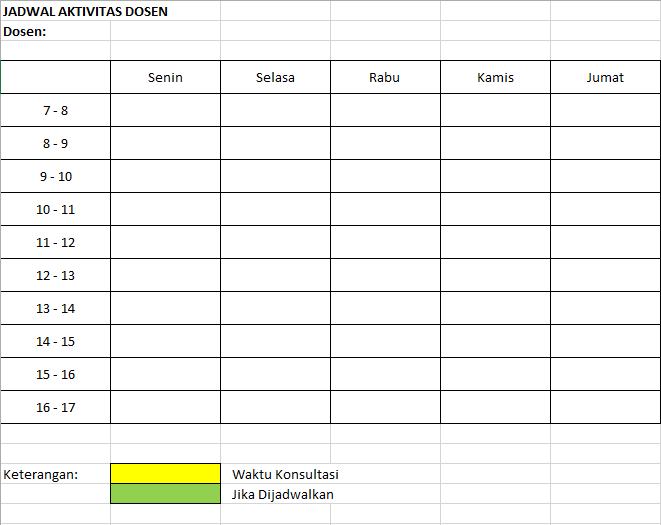
\includegraphics[scale=0.7]{template-jadwal-dosen.png}
\begin{figure} [h]
	\centering  
	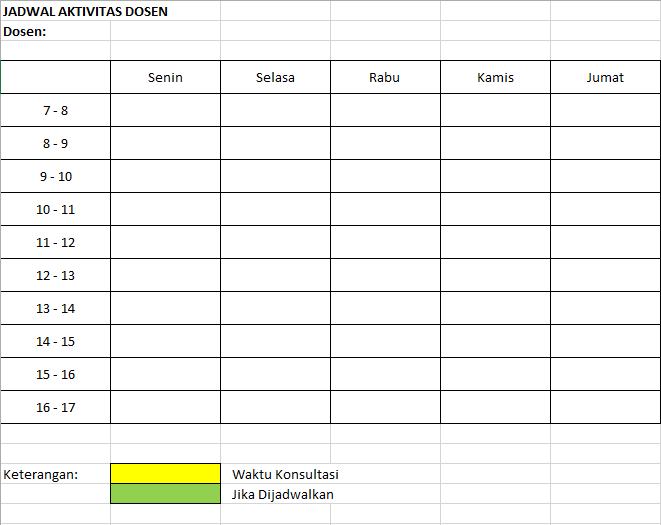
\includegraphics[scale=0.5]{template-jadwal-dosen.png}  
	\caption[Template jadwal dosen]{Template jadwal dosen} 
	\label{fig:template-jadwal-dosen} 
\end{figure} 
Jadwal tersebut akan ditempel pada dinding ruangan masing-masing dosen. Sedangkan bila menggunakan Blue Tape maka dosen tidak perlu lagi mencetak jadwalnya tersebut karena mahasiswa dapat melihat jadwal setiap dosen di dalam aplikasi ini. Maka dari itu aplikasi ini membuat pencatatan jadwal dosen menjadi \textit{papeless}.

%referensi pake unpublished

Pada Skripsi ini akan ditambahkan dua modul yaitu modul entri jadwal untuk dosen informatika dan modul lihat jadwal dosen untuk mahasiswa ke dalam aplikasi Blue Tape. Modul-modul tersebut berfungsi untuk melakukan hal-hal yang berhubungan dengan pembangkitan jadwal dosen. Modul dosen memiliki beberapa fungsi diantarnya: input jadwal mingguan dosen(jadwal dapat berupa jadwal konsultasi, jadwal konsultasi tentatif ataupun jadwal rutin), mencatat \textit{update} terakhir jadwal dosen dan mengekspor jadwal dosen ke XLS. Modul Umum sendiri memiliki fungsi untuk melihat jadwal seluruh dosen dan mengekspor jadwal dosen ke XLS.


\section{Rumusan Masalah}
\label{sec:rumusan}
Rumusan masalah yang akan dibahas dalam penelitian ini :
	\begin{enumerate}
		\item Bagaimana cara mencatat, \textit{update} dan melihat jadwal dosen di \textit{Blue Tape}?
		\item Bagaimana mengekspor jadwal dosen ke XLS sesuai template yang saat ini berlaku?
	\end{enumerate}


\section{Tujuan}
\label{sec:tujuan}
Tujuan yang ingin dicapai dalam penelitian ini : 
	\begin{enumerate}
		\item Membuat modul entri jadwal dosen dan modul lihat jadwal dosen yang berfungsi untuk menginput jadwal mingguan, \textit{update} dan melihat jadwal dosen
		\item Mengimplementasikan kode-kode yang diperlukan untuk memasukkan data yang ada di dalam PHP ke dalam \textit{file} XLS. 

	\end{enumerate}

\section{Batasan Masalah}
\label{sec:batasan}
Dalam penelitian ini ditetapkan batasan-batasan masalah sebagai berikut:
\begin{enumerate}
	\item Aplikasi ini tidak memeriksa hasil akhir bertipe file .xls, .xlsx atau tipe file lainnya.
	\item Aplikasi ini tidak mendukung fitur \textit{drag and drop}
	\item Aplikasi ini tidak mendukung fitur pemasukan jadwal dari sumber eksternal.
\end{enumerate}

\section{Metodologi}
\label{sec:metlit}
Metode penelitian yang akan digunakan dalam skripsi ini adalah:
\begin{enumerate}
   \item Studi literatur mengenai:
   		\begin{enumerate}
 		\item bahasa pemrograman PHP
 		\item \textit{framework} Codeigniter
 		\item modul \textit{Zurb Foundation} dan PHPExcel
		\end{enumerate}
   \item Analisis kebutuhan aplikasi dengan mengenali metode pencatatan jadwal dosen saat ini dan mengimplementasikannya ke dalam modul tersebut
    \item Membangun modul aplikasi yang sesuai dengan kebutuhan dosen dan mahasiswa dalam pembangkitan jadwal dosen agar aplikasi yang dibuat dapat membantu kedua pihak dalam mengakses informasi-informasi yang berkaitan dengan jadwal dosen . Pembuatan modul aplikasi ini dibagi menjadi empat tahap :
    	\begin{enumerate}
 		\item Analisis kebutuhan modul 
 		\item Perancangan modul
 		\item Implementasi 
 		\item Pengujian modul
		\end{enumerate}
\end{enumerate}
 

\section{Sistematika Pembahasan}
\label{sec:sispem}
Untuk penulisan skripsi ini akan dibagi dalam enam bagian sebagai berikut :

Bab 1 Pendahuluan berisi latar belakang, rumusan masalah, tujuan, batasan masalah,  metodologi penelitian dan sistematika penulisan.

Bab 2 Landasan Teori berisi dasar-dasar teori yang akan digunakan dalam pembuatan aplikasi pembangkit jadwal dosen. Dasar-dasar teori yang akan digunakan diantarnya adalah bahasa pemrograman PHP, framework Codeigniter, Google OAuth, CSRF, Zurb Foundation dan PHPExcel.

Bab 3 Analisis berisi analisis kebutuhan data, analisis sistem yang sudah ada sekarang dan analisis sistem usulan.

Bab 4 Perancangan berisi perancangan basis data, perancangan kelas-kelas program dan perancangan antarmuka program.

Bab 5 Implementasi dan Pengujian menjelaskan mengenai lingkungan yang digunakan dalam proses implementasi dan pengujian Aplikasi Pembangkit Jadwal Dosen. Bab ini juga mencatat hasil pengujian fungsional dan hasil pengujian eksperimental program.

Bab 6 Kesimpulan dan Saran berisi kesimpulan dari hasil pembuatan Aplikasi Pembangkit Jadwal Dosen ini dan kegunaannya, serta memberikan saran-saran untuk kelanjutan pengembangan aplikasi ini.
